\begin{figure*}[!t]
\centering
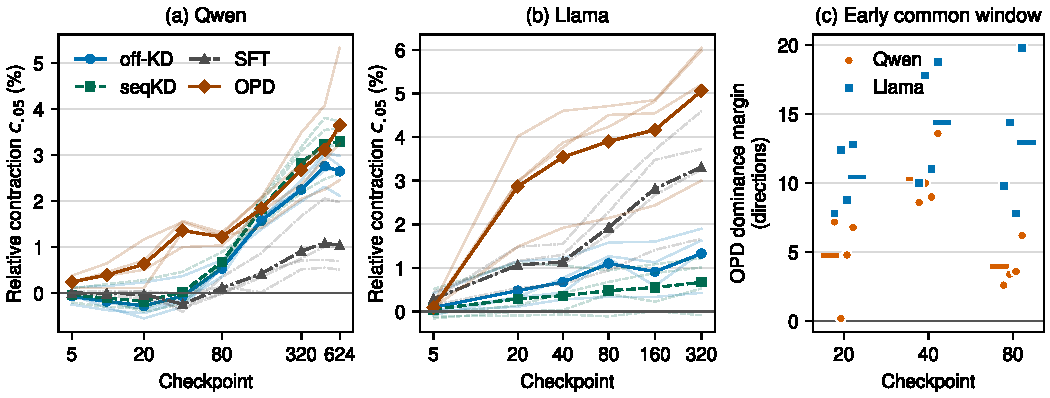
\includegraphics[width=\textwidth]{figures/fig1_main_trajectories.pdf}
\caption{Activation, weight, and functional trajectories. Rows show Qwen and Llama;
columns show activation ER, TPNT excess lift above its null, PABS drift
$10^4(1-\mathrm{PABS})$, and equal-5 relative functional contraction. Column scales have
different units and raw magnitudes are not comparable. Lines connect observed checkpoints
only. Functional contraction exposes training-setting separation not jointly reproduced
by the preceding coordinates.}
\label{fig:main}
\end{figure*}

\begin{table*}[!t]
\centering
\small
\setlength{\tabcolsep}{5pt}
\begin{tabular}{lccc}
\toprule
Model & Activation suite $A$ & Functional $C_5$ & Weight $P_{k,5}$ \\
\midrule
Llama & .556 & \textbf{.743} & .688 \\
Qwen & .595 & \textbf{.708} & .521 \\
\bottomrule
\end{tabular}
\caption{OPD identification on strict common grids (checkpoint-held-out AUC). Each model
uses 64 common states, identical equal-5 modules, and identical folds. $A$ is the
eight-feature activation suite containing ER, PR, top-1/8/32 shares, raw/centered
anisotropy, and step-0 CKA; it is not the single ER trajectory in Figure~\ref{fig:main}.}
\label{tab:identification}
\end{table*}

\begin{table*}[!t]
\centering
\small
\setlength{\tabcolsep}{4pt}
\begin{tabular}{lrrrrr}
\toprule
Model & $M_{\min}^{\mathrm{early}}$ & OPD NCD & SFT NCD & off-KD NCD & seqKD NCD \\
\midrule
Qwen & .200 & \textbf{50.423} & 9.554 & 31.017 & 37.793 \\
Llama & 7.800 & \textbf{77.594} & 39.683 & 17.518 & 11.093 \\
\bottomrule
\end{tabular}
\caption{Shared early ordering and full-trajectory contraction dose.
$M_{\min}^{\mathrm{early}}$ is the minimum continuous OPD margin over four core domains
and shared early checkpoints (directions); positivity excludes a reversal on this grid.
NCD integrates depth and duration through $T=320$ in directions$\times$log-step. The
two columns have different units and are not numerically comparable.}
\label{tab:ncd}
\end{table*}

\begin{figure*}[!t]
\centering
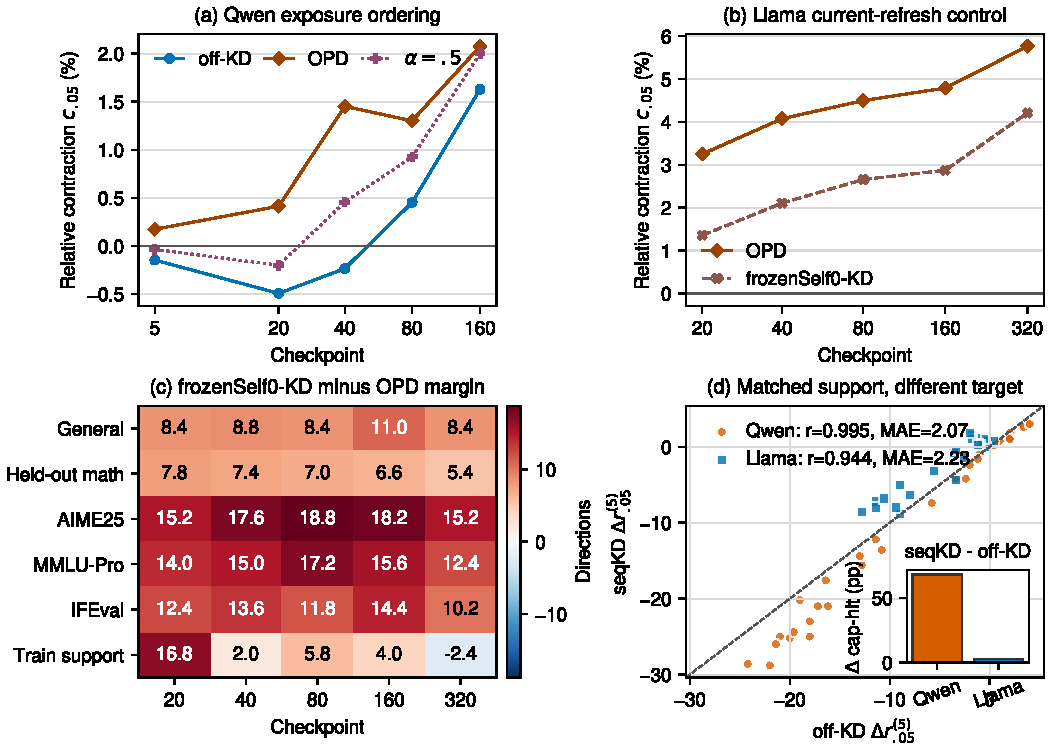
\includegraphics[width=\textwidth]{figures/fig2_support_controls.pdf}
\caption{Sequence-exposure and refresh controls. (a) Ordered Qwen $\alpha=.5$ movement
relative to off-KD and OPD. (b) Mean absolute trajectories of Llama OPD and
frozenSelf0-KD over five fixed external domains. (c) Corresponding paired margins;
positive values indicate deeper contraction under continuously refreshed OPD, and the
thick black line is the external-domain mean. Math, AIME, MMLU, and Mean denote held-out
math, AIME25, MMLU-Pro, and the five-domain mean.}
\label{fig:controls}
\end{figure*}

\begin{table*}[!t]
\centering
\small
\setlength{\tabcolsep}{2.7pt}
\textbf{A. Per-domain equal-5 path agreement, off-KD vs. seqKD
(Pearson $r$/MAE directions)}\\[2pt]
\begin{tabular}{lccccc}
\toprule
Model & General & Math & MMLU-Pro & IFEval & Pooled \\
\midrule
Qwen & .995/1.13 & .996/2.67 & .998/2.18 & .999/2.29 & .995/2.07 \\
Llama & -.771/2.53 & .971/1.73 & .968/2.23 & .824/2.40 & .944/2.23 \\
\bottomrule
\end{tabular}

\vspace{4pt}
\textbf{B. Endpoint behavior for matched-support settings (\%)}\\[2pt]
\begin{tabular}{llrrrrrrr}
\toprule
Model & Setting & \multicolumn{2}{c}{MATH500} & \multicolumn{3}{c}{MMLU-Pro} & \multicolumn{2}{c}{IFEval} \\
\cmidrule(lr){3-4}\cmidrule(lr){5-7}\cmidrule(lr){8-9}
 & & Acc. & Cap & Strict & Flex. & Extract & Prompt & Instr. \\
\midrule
Qwen & off-KD & 79.4 & 4.8 & 35.4 & 57.1 & 47.3 & 23.1 & 36.5 \\
 & seqKD & 72.4 & 73.0 & 30.6 & 58.1 & 54.1 & 24.4 & 39.3 \\
Llama & off-KD & 8.2 & 91.8 & 14.2 & 16.4 & 50.3 & 19.6 & 33.2 \\
 & seqKD & 10.2 & 94.6 & 13.1 & 15.4 & 51.6 & 19.2 & 31.5 \\
\bottomrule
\end{tabular}
\caption{Matched-support functional paths and behavioral readout. A uses matched nonzero
checkpoints; MAE is the checkpoint-wise direction difference. B uses Qwen step 624 and
Llama step 320. Cap denotes generation-cap hit, Extract extraction failure, and
Prompt/Instr. IFEval prompt/instruction strict.}
\label{tab:support-readout}
\end{table*}

\begin{figure*}[!t]
\centering
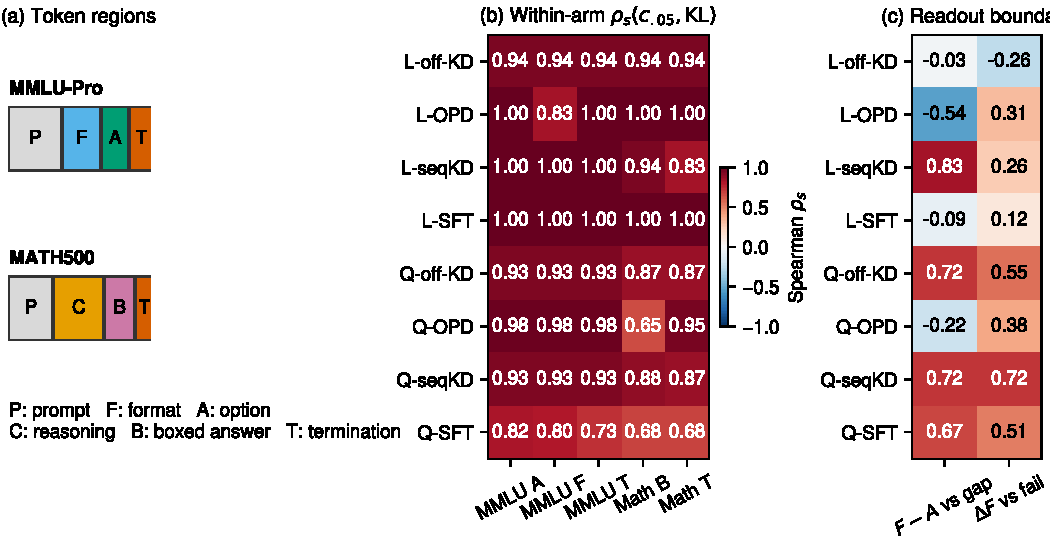
\includegraphics[width=\textwidth]{figures/fig3_regional_output.pdf}
\caption{Regional output relationships. (a) Within-model, within-setting Spearman
correlations between equal-5 functional contraction and regional full-vocabulary KL.
MMLU-Pro columns are format ($F$), correct answer-choice label ($A$), and termination
($T$); MATH500 columns are reasoning ($C$), boxed answer ($B$), and termination ($T$).
(b) MMLU-Pro correlations of the format--answer signed-NLL contrast with the
strict--flexible gap and of format NLL with extraction failure. L and Q denote Llama and
Qwen; each cell prints its correlation.}
\label{fig:regional}
\end{figure*}

\begin{table*}[!t]
\centering
\small
\setlength{\tabcolsep}{4pt}
\begin{tabular}{llcc}
\toprule
Model/domain & Regions & Held-out $R^2$: $C_5$ & Best $P_{k,5}$ \\
\midrule
Llama / MMLU-Pro & $A/F/T$ & \textbf{.869/.932/.468} & .743/.788/.459 \\
Llama / MATH500 & $B/T$ & .561/\textbf{.812} & \textbf{.615}/.647 \\
Qwen / MMLU-Pro & $A/F/T$ & \textbf{.426/.577/.596} & .243/.318/.443 \\
Qwen / MATH500 & $B/T$ & \textbf{.227}/.604 & .167/\textbf{.718} \\
\bottomrule
\end{tabular}
\caption{Out-of-fold prediction of regional full-vocabulary KL. $C_5$ and $P_{k,5}$
use the same five modules, states, and checkpoint-held-out folds. Values follow the
region order; bold marks the higher per-region $R^2$. The later Math $C$ audit is
reported within trajectories and after checkpoint demeaning, but is not included in
this matched held-out table.}
\label{tab:regional-prediction}
\end{table*}
